\documentclass{sigchi}

% Use this command to override the default ACM copyright statement
% (e.g. for preprints).  Consult the conference website for the
% camera-ready copyright statement.

%% EXAMPLE BEGIN -- HOW TO OVERRIDE THE DEFAULT COPYRIGHT STRIP -- (July 22, 2013 - Paul Baumann)
% \toappear{Permission to make digital or hard copies of all or part of this work for personal or classroom use is      granted without fee provided that copies are not made or distributed for profit or commercial advantage and that copies bear this notice and the full citation on the first page. Copyrights for components of this work owned by others than ACM must be honored. Abstracting with credit is permitted. To copy otherwise, or republish, to post on servers or to redistribute to lists, requires prior specific permission and/or a fee. Request permissions from permissions@acm.org. \\
% {\emph{CHI'14}}, April 26--May 1, 2014, Toronto, Canada. \\
% Copyright \copyright~2014 ACM ISBN/14/04...\$15.00. \\
% DOI string from ACM form confirmation}
%% EXAMPLE END -- HOW TO OVERRIDE THE DEFAULT COPYRIGHT STRIP -- (July 22, 2013 - Paul Baumann)

% Arabic page numbers for submission.  Remove this line to eliminate
% page numbers for the camera ready copy
% \pagenumbering{arabic}

% Load basic packages
\usepackage{balance}  % to better equalize the last page
\usepackage{graphics} % for EPS, load graphicx instead 
\usepackage{txfonts}
\usepackage{mathptmx}
\usepackage[pdftex]{hyperref}
\usepackage{color}
\usepackage{booktabs}
\usepackage{textcomp}
\usepackage{microtype} % Improved Tracking and Kerning
\usepackage{ccicons}  % Cite your images correctly!

\usepackage[T1]{fontenc}
\usepackage[utf8]{inputenc}
\usepackage[ngerman]{babel}

%\usepackage[ansinew]{inputenc}
%\usepackage[T3]{fontenc}
\usepackage{todonotes}

% Paper metadata (use plain text, for PDF inclusion and later
% re-using, if desired).  Use \emtpyauthor when submitting for review
% so you remain anonymous.
\def\plaintitle{Parallel World}
\def\plainauthor{First Author, Second Author, Third Author,
  Fourth Author, Fifth Author, Sixth Author}
\def\emptyauthor{}
\def\plainkeywords{Authors' choice; of terms; separated; by
  semicolons; include commas, within terms only; required.}
\def\plaingeneralterms{Documentation, Standardization}

% llt: Define a global style for URLs, rather that the default one
\makeatletter
\def\url@leostyle{%
  \@ifundefined{selectfont}{
    \def\UrlFont{\sf}
  }{
    \def\UrlFont{\small\bf\ttfamily}
  }}
\makeatother
\urlstyle{leo}

% To make various LaTeX processors do the right thing with page size.
\def\pprw{8.5in}
\def\pprh{11in}
\special{papersize=\pprw,\pprh}
\setlength{\paperwidth}{\pprw}
\setlength{\paperheight}{\pprh}
\setlength{\pdfpagewidth}{\pprw}
\setlength{\pdfpageheight}{\pprh}

% Make sure hyperref comes last of your loaded packages, to give it a
% fighting chance of not being over-written, since its job is to
% redefine many LaTeX commands.
\definecolor{linkColor}{RGB}{6,125,233}
\hypersetup{%
  pdftitle={\plaintitle},
% Use \plainauthor for final version.
%  pdfauthor={\plainauthor},
  pdfauthor={\emptyauthor},
  pdfkeywords={\plainkeywords},
  bookmarksnumbered,
  pdfstartview={FitH},
  colorlinks,
  citecolor=black,
  filecolor=black,
  linkcolor=black,
  urlcolor=linkColor,
  breaklinks=true,
}

% create a shortcut to typeset table headings
% \newcommand\tabhead[1]{\small\textbf{#1}}

% End of preamble. Here it comes the document.
\begin{document}

\title{\plaintitle}

\numberofauthors{3}
\author{%
  \alignauthor{Daniel Graf\\
    \affaddr{Hochschule München}\\
    \affaddr{München}\\
    \email{graf12@hm.edu}}\\
  \alignauthor{Ludwig Wagner\\
    \affaddr{Hochschule München}\\
    \affaddr{München}\\
    \email{wagner43@hm.edu}}\\
  \alignauthor{Dimitrie Diez\\
    \affaddr{Hochschule München}\\
    \affaddr{München}\\
    \email{diez@hm.edu}}\\
}

\maketitle

\begin{abstract}
% In der heutigen Zeit gibt es viele verschiedene Authentifizierungsverfahren, die den Menschen vertraut sind. Der Mensch nutzt heute verschiedene Plattformen und Devices um Informationen aufzubewahren oder mit anderen Personen zu teilen. Der Zugang zu diesen Daten muss durch Authentifizierungsverfahren bestmöglich geschützt werden. Die am häufigsten verwendeten Methoden sind E-Mail Adresse und Passwort. Bei zahlreichen Onlineplattformen, wie beispielsweise Yahoo, SchülerVZ oder Sony wurden Millionen Kundendatensätze gestohlen und im Darknet veröffentlicht. Somit fehlen Angreifern lediglich die Passwörter um in die Accounts zu gelangen. Angreifer versuchen häufig diese durch BruteForce Angriffe zu ermitteln. Dies ist möglich, da der Angreifer bei fehlerhaften Login Informationen informiert wird. Um dies zu verhindern wurde ein Konzept für einen Authentifizierungsvorgang entwickelt, bei dem der Angreifer genau diese Informationen nicht erhält. Das Konzept wurde für Social Networks ausgelegt, ist jedoch vielseitig, beispielsweise auch für E-Mail Accounts, verwendbar. Bei einem fehlgeschlagenen Authentifizierungsvorgang wird ein erfolgreicher Login, durch die Anzeige eines täuschend echt aussehenden Fake-Kontos, vorgetäuscht. Für die Umsetzung des Konzepts wurden verschiedene Handlungsempfehlungen erarbeitet und limitierende Faktoren aufgezeigt. Basierend auf diesen Aspekten erfolgt eine Bewertung des Konzepts hinsichtlich Sicherheit, Umsetzbarkeit und Benutzbarkeit. 
% 
%
%\todo[inline]{Paper: Aspekte die berücksichtigt werden müssen damit man es bauen kann bzw. Empfehlungen zum bauen des Projekts (Bewertung des Konzept im Paper)
%	Paper: Ausarbeitung welche Teilkonzepte am erfolgversprechendsten sind, welche sind nicht machbar; AUS BENUTZERSICHT}
%  KONZEPT dagegen ...   Durch ein geschicktes Konzept wird dieser Angriffsvektor unterbunden. Konzept ursprünglich für Social Network jedoch vielseitig verwendbar
%Es lohnt sich nicht ein eigenes Netzwerk mit dem Konzept zu entwickeln
%Viele Leute sind nicht bereit
\end{abstract}

%\category{H.5.m.}{Information Interfaces and Presentation
%  (e.g. HCI)}{Miscellaneous} \category{See
%  \url{http://acm.org/about/class/1998/} for the full list of ACM
%  classifiers. This section is required.}{}{}
%
%\keywords{\plainkeywords}

\section{Einlüitung}
Einleitung mit einer Statistik über Angriffe und Sicherheitslücken aktueller Social Media Plattformen, Identifikation des Problems bei aktuellen Authentifizierungsverfahren (Der Angreifer weiss, dass Login fehlgeschlagen ist)

\section{Weiterführende Literatur}
%jeder sucht Literatur zu diesem Thema und beschreibt Ergebnis in einem bis zwei Sätzen. Was haben andere rausgefunden?
%ISBN: 978-1-4799-6364-5 (IEEE Passwords are Dead)

 
\section{Beschreibung des Konzepts}

Kernpunkt des Konzept ist die Erschaffung eines parallelen Fake-Netzwerkes. Dadurch soll verhindert werden, dass ein Angreifer in das Netzwerk gelangt oder Informationen über die Mitglieder des Netzwerkes gewinnen kann. Im folgenden wird der Aufbau des Netzwerkes anhand eines Login-Vorgangs beschrieben. \\
Auf der Startseite des Netzwerkes werden die Nutzer zunächst aufgefordert E-Mail Adresse und Passwort einzugeben, bevor sie zum zweiten Schritt der Authentifizierung gelangen. Hierfür muss jeder Nutzer bei der Registrierung eines, oder mehrere Authentifizierungsverfahren hinterlegen. Zur Auswahl stehen einen Authentifizierung mittels eines Codes, welcher per SMS zugesandt wird, mittels Push-Benachrichtigung am Mobiltelefon oder mittels biometrischer Daten. Unabhängig davon, ob E-Mail Adresse, Passwort, die Wahl des Verfahrens oder die Durchführung des Verfahrens korrekt waren, gelangt der Nutzer in das Netzwerk. Doch nur im Falle eines vollständig korrekten Vorgangs befindet sich der Nutzer in seinem Account im "echten" Netzwerk. Andernfalls gelangt der Nutzer in ein täuschend echt aussehendes Fake-Profil, welches nur vom Inhaber als solches enttarnt werden kann. Der Angreifer erfährt dadurch weder ob seine eingegebenen Angaben korrekt waren bzw. welche nicht korrekt waren, noch kann er sich sicher sein, ob er im echten Netzwerk ist. Sämtliche, für ihn sichtbaren Informationen sind folglich nicht verifizierbar und daher nahezu wertlos. \\
Die größte Herausforderung bei der Umsetzung des Konzeptes stellt die Generierung des Fake-Netzwerkes dar. Hierfür wurden 4 unterschiedliche Umsetzungsvarianten definiert, welche im Folgenden beschrieben werden. \\
In der ersten Variante, muss jeder Nutzer bei der Registrierung neben seinem echten Profil auch ein Fake Profil anlegen. Welche Informationen er hierfür verwendet, ist ihm überlassen. 
\begin{minipage}{\columnwidth}
%	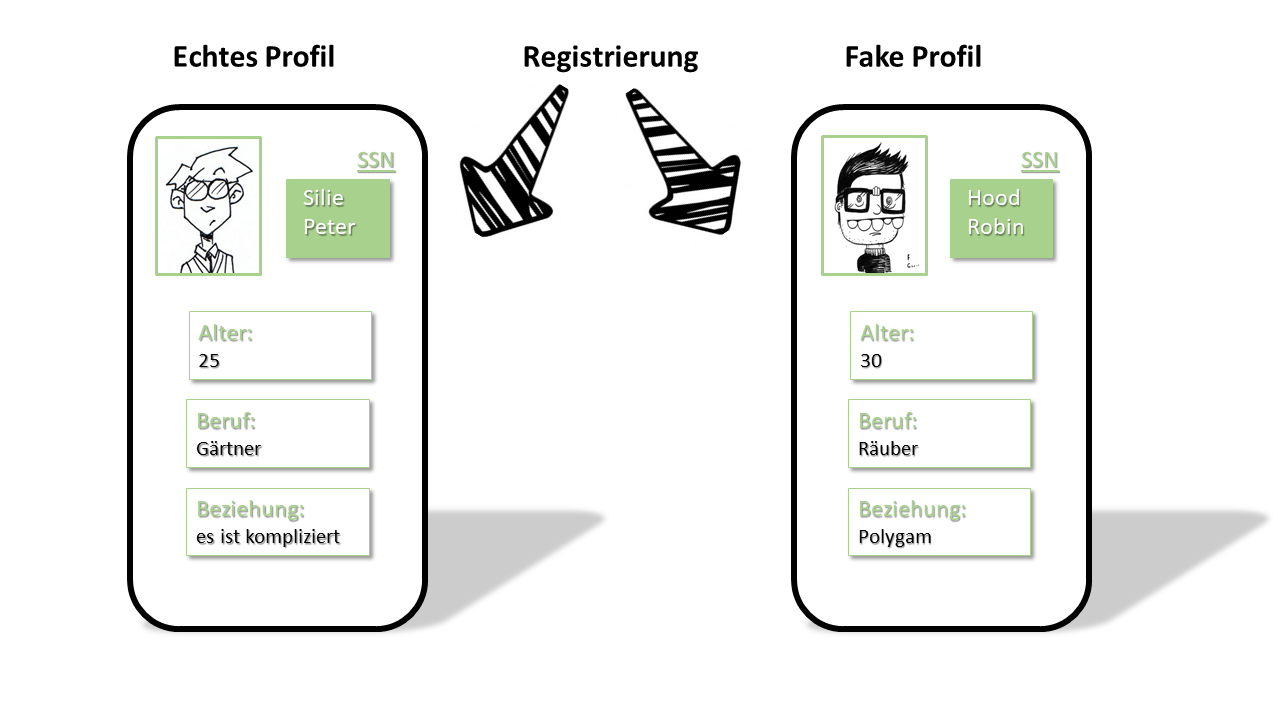
\includegraphics[width=0.8\columnwidth]{Umsetzung1.jpeg}
	\centering
%	\captionof{figure}{Test}
	\label{fig:ASIL}
\end{minipage}
\\
In der zweiten Variante erstellt der Nutzer lediglich sein echtes Profil. Er kann jedoch für jede Information, beispielsweise dem Namen, seinem Alter oder dem Profilbild durch setzen eines Hakens entscheiden, ob diese Information für die Erstellung des Fake-Profils verwendet werden darf, oder nicht. Restliche Daten werden durch das System zufällig generiert.  BILD \\
In der dritten Variante werden alle Fake-Profile automatisch generiert. Die Nutzer können den Prozess hierbei nicht beeinflussen. BILD \\
In der vierten Variante werden die Fake-Profile, analog zu Variante 3 automatisch generiert. Hierbei wird der Nutzer jedoch aufgefordert Bilder für die Fake-Profil Generierung zur Verfügung zu stellen. Dadurch soll erreicht werden, dass die Fake-Profile für einen Angreifer authentischer Wirken. BILD \\

\section{Methodik}

\subsection{Fokusgruppe}
Aufbau der Umfrage, des Experimentes... 
\subsection{Einzelbefragungen}
Aufbau der Umfrage, des Experimentes... 

\subsection{Ergebnisse}
auch das Mindmap reinnehmen... Oder CLusterbildung... usw.

\subsection{Diskussion der Herausforderungen bei der Umsetzung des Konzepts}
Ergebnisse von Fokusgruppe + Einzelbefragungen, Diskussion der wichtigsten Aspekte  
\subsection{Handlungsempfehlungen}
Lösungsansätze der vorher beschriebenen Probleme vorstellen. + Diskussion der Umsetzbarkeit
\subsubsection{Speichern des Logins}
Mechanismen, die es erlauben Logins temporär zu speichern sind State of The Art. Diese Mechanismen müssen auch bei diesem Konzept angewendet werden um eine akzeptable Usability zu gewährleisten.
\subsubsection{Integration in ein bestehendes Sozial Network statt Entwicklung eines neuen}
Da Nutzer sich nicht wegen dem Sicherheitskonzept in einem Netzwerk registrieren, sondern wegen Kontakten soll das Konzept in ein bestehendes Netzwerk integriert werden und kein neues Netzwerk entwickelt werden.
\subsubsection{Klare Erläuterung des Sicherheitskonzeptes}
Durch attraktiv gestaltete Grafiken, Illustrationen, Videos oder Tutorials muss der Benutzer in kurzer Zeit über die Vorteile des Konzepts informiert werden.
\subsubsection{Automatische und manuelle Fakeprofil Erstellung}
Die Fakeprofil Erstellung muss automatisiert erfolgen. Den Nutzern muss die Möglichkeit gegeben werden Daten für die Generierung des Fake Profils zur Verfügung zu stellen. Den Nutzern muss bewusst gemacht werden, dass die Fake Profile durch die Angaben persönlicher (echter) Daten authentischer wirken.
\subsubsection{Umgang mit Passwortverlust}
Das Zurücksetzen des Passworts muss möglich sein.
\subsubsection{Auswahl unterschiedlicher Verfahren für die 2-Wege Authentifizierung}
Dem Nutzer muss eine große Anzahl an hinterlegbaren Authentifizierungsmechanismen zur Auswahl gestellt werden
\subsubsection{Kommunikation im Netzwerk}
Die Kommunikation mit Fake Profilen muss möglich sein. Das suchen von Profilen muss möglich sein. Aus Fake Profilen müssen alle Aktionen möglich sein, die auch mit echten Profilen getätigt werden können.
\section{Zusammenfassung und Fazit}
Was wurde gemacht, Handslungsempf zusammenfassen..
Die Wichtigsten erläutern
\section{Ausblick}

% REFERENCES FORMAT
% References must be the same font size as other body text.
%\bibliographystyle{SIGCHI-Reference-Format}
%\bibliography{sample}

\end{document}

%%% Local Variables:
%%% mode: latex
%%% TeX-master: t
%%% End:
